\documentclass[12pt]{extarticle}
\usepackage{tempora}
\usepackage[T1, T2A]{fontenc}
\usepackage[utf8]{inputenc}
\usepackage[english, ukrainian]{babel}
\usepackage{geometry}
\usepackage{graphicx}
\usepackage{multirow}
\usepackage{multicol}
\usepackage{float}
\usepackage{tikz}
\graphicspath{{/home/artem/Pictures}}
\geometry
{
    a4paper,
    left=30mm,
    top=15mm,
    right=20mm,
    bottom=15mm,
}

\begin{document}
\begin{titlepage}
    \begin{center}
        \textbf{\normalsize{\MakeUppercase{
            Міністерство Освіти і науки України
            Національний університет "Львівська політехніка"
        }}}

        \begin{flushright}
        \textbf{ІКНІ}\\
        Кафедра \textbf{ПЗ}
        \end{flushright}
        \vspace{15mm}

        \includegraphics[width=0.4\textwidth]{lpnu_logo.png}

        \vspace*{\fill}

        \textbf{\normalsize{\MakeUppercase{Звіт}}}
            
        До розрахункової роботи №1

        \textbf{на тему:} “Мінімізація логічних функцій. Синтез комбінаційних схем”

        \textbf{з дисципліни:} “Архітектура комп’ютера”
            
        \vspace*{\fill}

        \begin{flushright}

            %\textbf{Лектор:}\\
            %доцент кафедри ПЗ\\
            %Крук О.Г.\\
            %\vspace{12pt}

            \textbf{Виконав:}\\
            студент групи ПЗ-24\\
            Губик А. С.\\
            \vspace{12pt}

            %\textbf{Прийняв:}\\
            %доцент кафедри ПЗ\\
            %Задорожний І. М.\\
        \vspace{12pt}
        \end{flushright}

        Львів -- 2023
            
            
    \end{center}
\end{titlepage}

\vspace{12pt}

\subsection*{Індивідуальне завдання}

\begin{center}
    \begin{tabular}{| c | c | c | c | c |}
    \hline
    $x_4$ & $x_3$ & $x_2$ & $x_1$ & $y$\\
    \hline
    0 & 0 & 0 & 0 & 1\\
    \hline
    0 & 0 & 0 & 1 & 0\\
    \hline
    0 & 0 & 1 & 0 & 1\\
    \hline
    0 & 0 & 1 & 1 & 1\\
    \hline
    0 & 1 & 0 & 0 & 1\\
    \hline
    0 & 1 & 0 & 1 & 0\\
    \hline
    0 & 1 & 1 & 0 & 1\\
    \hline
    0 & 1 & 1 & 1 & 1\\
    \hline
    1 & 0 & 0 & 0 & 0\\
    \hline
    1 & 0 & 0 & 1 & 0\\
    \hline
    1 & 0 & 1 & 0 & 1\\
    \hline
    1 & 0 & 1 & 1 & 1\\
    \hline
    1 & 1 & 0 & 0 & 0\\
    \hline
    1 & 1 & 0 & 1 & 0\\
    \hline
    1 & 1 & 1 & 0 & 1\\
    \hline
    1 & 1 & 1 & 1 & 0\\
    \hline
    \end{tabular}
\end{center}

\subsection*{Хід роботи}
\paragraph{1.}
ДДНФ відповідно до індивідуального завдання:

$( \bar x_4 \land \bar x_3 \land \bar x_2 \land \bar x_1) \lor$

$( \bar x_4 \land \bar x_3 \land  x_2 \land x_1) \lor$

$( \bar x_4 \land \bar x_3 \land x_2 \land \bar x_1) \lor$

$( \bar x_4 \land x_3 \land \bar x_2 \land \bar x_1) \lor$

$( \bar x_4 \land x_3 \land x_2 \land \bar x_1) \lor$

$( \bar x_4 \land x_3 \land x_2 \land x_1) \lor$

$( x_4 \land \bar x_3 \land x_2 \land \bar x_1) \lor$

$( x_4 \land \bar x_3 \land x_2 \land x_1) \lor$

$( x_4 \lor x_3 \lor x_2 \lor \bar x_1). $

\paragraph{2.}
Карта Карно:

\begin{center}
    \begin{tabular}{| c | c | c | c | c |}
    \hline
    & $x_4x_3$ & $x_4 \bar x_3$ & $\bar x_4 \bar x_3$ & $\bar x_4x_3$\\
    \hline
    $x_2  x_1$          & 1 &   & 1 & 1\\
    \hline
    $x_2 \bar x_1$      & 1 &   & 1 & 1\\
    \hline
    $\bar x_2 \bar x_1$ &   &   &   & 1\\
    \hline
    $\bar x_2 x_1$      &   &   & 1 & 1\\
    \hline
    \end{tabular}

    \begin{tikzpicture}[overlay]
        \draw[black, line width=1.0pt] (1.8,1.65) ellipse (1cm and 0.6cm);
        \draw[black, line width=1.0pt] (1.85,0.3) ellipse (1.1cm and 0.3cm);
        \draw[black, line width=1.0pt] (-1.23,1.65) ellipse (0.2cm and 0.5cm);
        %\draw[black, line width=1.0pt] (1.23,0.3) ellipse (0.2cm and 0.5cm);
        \draw[black, line width=1.0pt] (2.46,1.1) ellipse (0.2cm and 1.1cm);
    \end{tikzpicture} 
    
\end{center}
\vspace{12pt}
Тоді функція $F_{min_1}$:

$ \bar x_4 \bar x_1 \lor 
  \bar x_4 x_3 \lor 
   x_3 \bar x_2 \lor 
   x_3 \bar x_1. $

\break
\paragraph{3.}
Спрощення методом Квайна-Маккласкі:

\begin{center}
    \begin{tabular}{ c  c  c  c  }
    0 & 0 & 0 & 0 \\
    \hline
    0 & 0 & 1 & 0 \\
    0 & 1 & 0 & 0 \\
    \hline
    0 & 0 & 1 & 1 \\
    0 & 1 & 1 & 0 \\
    1 & 0 & 1 & 0 \\
    \hline
    0 & 1 & 1 & 1 \\
    1 & 0 & 1 & 1 \\
    1 & 1 & 1 & 0 \\
    \end{tabular}
    \hspace{1cm}
    \begin{tabular}{ c  c  c  c  }
    0 & 0 & -- & 0 \\
    0 & -- & 0 & 0 \\
    \hline
    0 & 0 & 1 & -- \\
    0 & -- & 1 & 0 \\
    -- & 0 & 1 & 0 \\
    0 & 1 & -- & 0 \\
    \hline
    0 & -- & 1 & 1 \\
    -- & 0 & 1 & 1 \\
    0 & 1 & 1 & -- \\
    -- & 1 & 1 & 0 \\
    1 & 0 & 1 & -- \\
    1 & -- & 1 & 0 \\
    \end{tabular}
    \hspace{1cm}
    \begin{tabular}{ c  c  c  c  }
    0 & -- & -- & 0 \\
    \hline
    0 & -- & 1 & -- \\
    -- & 0 & 1 & -- \\
    -- & -- & 1 & 0 \\
    \end{tabular}
\end{center}
Тоді функція $F_{min_2}$:

$ \bar x_4 \bar x_1 \lor 
  \bar x_4 x_3 \lor 
   x_3 \bar x_2 \lor 
   x_3 \bar x_1. $

\paragraph{4.}
ДКНФ:

$(  x_4 \lor  x_3 \lor  x_2 \lor \bar x_1) \land$

$(  x_4 \lor \bar x_3 \lor  x_2 \lor \bar x_1) \land$

$( \bar x_4 \lor  x_3 \lor x_2 \lor  x_1) \land$

$( \bar x_4 \lor x_3 \lor  x_2 \lor \bar x_1) \land$

$( \bar x_4 \lor \bar x_3 \lor x_2 \lor  x_1) \land$

$( \bar x_4 \lor \bar x_3 \lor x_2 \lor \bar x_1) \land$

$( \bar x_4 \lor \bar x_3 \lor \bar x_2 \lor \bar x_1) .$

\break
\paragraph{5.}
Схеми до функцій в Proteus:
\begin{figure}[H]
    \centering
    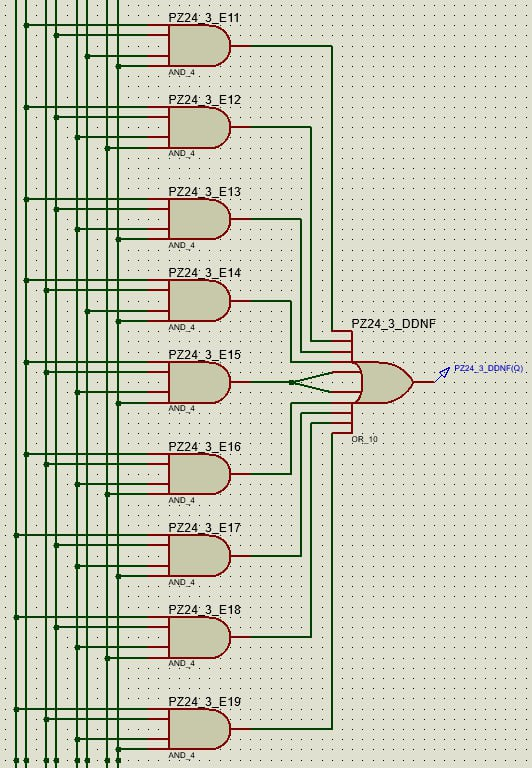
\includegraphics[width=0.90\textwidth]{ddnf.jpg}
    \caption{ДДНФ}
\end{figure}
\begin{figure}[H]
    \centering
    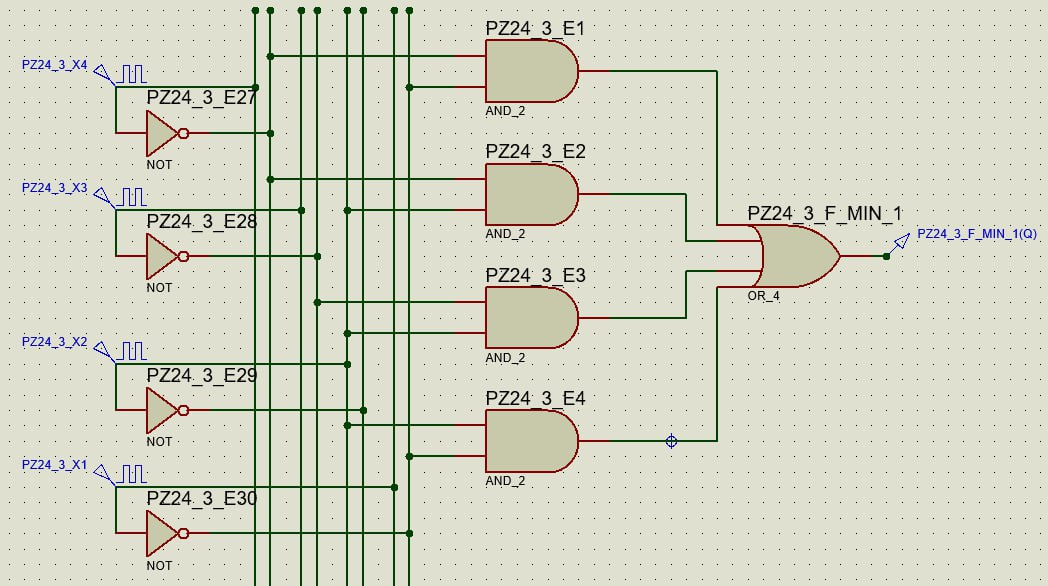
\includegraphics[width=0.90\textwidth]{f_min_1.jpg}
    \caption{Спрощена функція $F_{min_1}$}
\end{figure}
\begin{figure}[H]
    \centering
    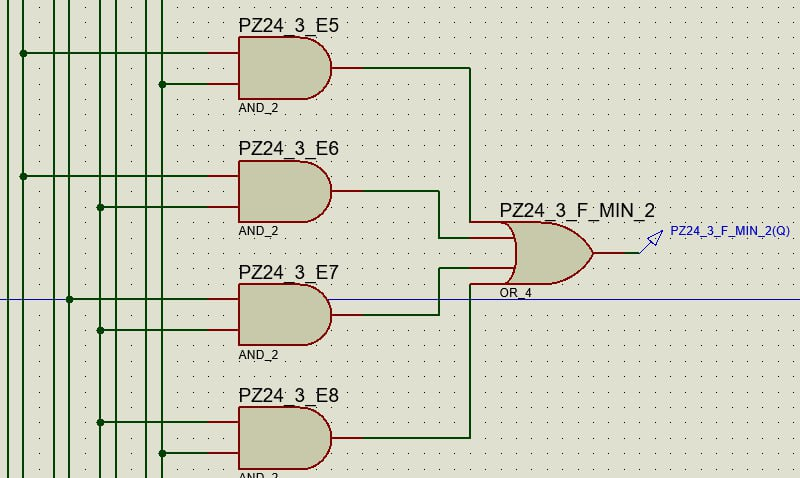
\includegraphics[width=0.90\textwidth]{f_min_2.jpg}
    \caption{Спрощена функція $F_{min_1}$}
\end{figure}
\begin{figure}[H]
    \centering
    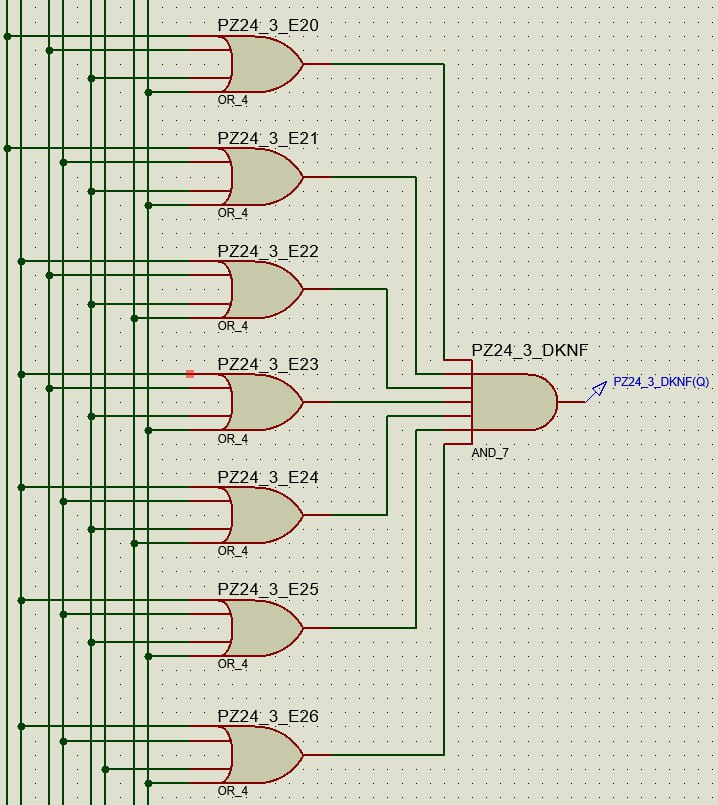
\includegraphics[width=0.90\textwidth]{dknf.jpg}
    \caption{ДКНФ}
\end{figure}
\begin{figure}[H]
    \centering
    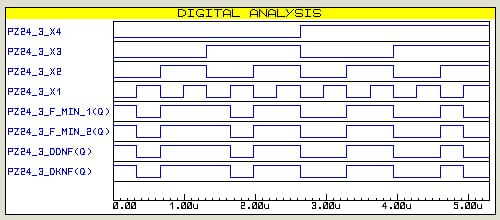
\includegraphics[width=0.90\textwidth]{graph.jpg}
    \caption{Графік функцій}
\end{figure}

\subsection*{Висновок}

Мінімізація логічних функцій дає змогу спростити функцію так, щоб 
в ній було менше змінних. Це дозволяє зменшити кількість елементів 
схеми, що робить її дешевшою, швидшою та надійнішою.

\end{document}